% Jeshua Kracht and Jacob Petrovic

\documentclass[conference]{IEEEtran}
%\makeindex
\usepackage{cite}
\usepackage{hyperref}
\usepackage[cmex10]{amsmath}
\usepackage{eqparbox}
%\usepackage[caption=false]{caption}
%\usepackage[font=footnotesize]{subfig}
\usepackage{url}
\usepackage{mathtools}
\usepackage[pdftex]{graphicx}
 
\begin{document}

\title{Comparing the Quality of Automatically Generated and Manually Written Test Suites}
% \subtitle{[Extended Abstract]}

\author{\IEEEauthorblockN{Jeshua Kracht, Jacob Z. Petrovic, \\Kristen R. Walcott-Justice}
\IEEEauthorblockA{Department of Computer Science\\
University of Colorado at Colorado Springs\\
Email: \{jkracht, jpetrovi, kjustice\}@uccs.edu}
%\and
%\IEEEauthorblockN{Jacob Z. Petrovic}
%\IEEEauthorblockA{Department of Computer Science\\
%University of Colorado at Colorado Springs\\
%Email: jpetrovi@uccs.edu}
%\and
%\IEEEauthorblockN{Kristen R. Walcott-Justice}
%\IEEEauthorblockA{Department of Computer Science\\
%University of Colorado at Colorado Springs\\
%Email: kjustice@uccs.edu}
\and
\IEEEauthorblockN{Ren\'{e} Just}
\IEEEauthorblockA{Computer Science \& Engineering\\
University of Washington\\
Email: rjust@cs.washington.edu}
\and
\IEEEauthorblockN{Gregory M. Kapfhammer}
\IEEEauthorblockA{Department of Computer Science\\
Allegheny College\\
Email: gkapfham@allegheny.edu}
}

%\author{\IEEEauthorblockN{Jeshua Krachtl\IEEEauthorrefmark{1},
%Jacob Z. Petrovic\IEEEauthorrefmark{2},
%Kristen R. Walcott-Justice\IEEEauthorrefmark{4}, and
%Gregory M. Kapfhammer\IEEEauthorrefmark{3}}
%\IEEEauthorblockA{\IEEEauthorrefmark{1}Department of Computer Science\\
%University of Colorado Colorado Springs\\
%Email: jkracht@uccs.edu}
%\IEEEauthorblockA{\IEEEauthorrefmark{2}Department of Computer Science\\
%University of Colorado Colorado Springs\\
%Email: jpetrovi@uccs.edu}
%\IEEEauthorblockA{\IEEEauthorrefmark{4}Department of Computer Science\\
%University of Colorado Colorado Springs\\
%Email: kjustice@uccs.edu}
%\IEEEauthorblockA{\IEEEauthorrefmark{3}Department of Computer Science\\
%Alleghent College\\
%Email: gkapfham@allegheny.edu}}
%Atlanta, Georgia 30332--0250\\ Email: see http://www.michaelshell.org/contact.html}
%\IEEEauthorblockA{\IEEEauthorrefmark{2}Twentieth Century Fox, Springfield, USA\\
%Email: homer@thesimpsons.com}
%\IEEEauthorblockA{\IEEEauthorrefmark{3}Starfleet Academy, San Francisco, California 96678-2391\\
%Telephone: (800) 555--1212, Fax: (888) 555--1212}
%\IEEEauthorblockA{\IEEEauthorrefmark{4}Tyrell Inc., 123 Replicant Street, Los Angeles, California 90210--4321}}

\maketitle
\begin{abstract}

\end{abstract}

% A category with the (minimum) three required fields
%\category{H.4}{Information Systems Applications}{Miscellaneous}
%A category including the fourth, optional field follows...
%\category{D.2.8}{Software Engineering}{Metrics}[complexity measures, performance measures]

% A category with the (minimum) three required fields
%What categories do we include?
%\category{D.2.5}{Software Engineering}{Testing and Debugging}{Testing tools}
%\category{D.2.8}{Software Engineering}{Software Metrics}{Performance measures}

%\terms{Measurement, Experimentation}

%\keywords{Mutation Testing, Test Suite, Mutation Score, Test Generation, Source Code, Mutant Operators, Infect, Code Coverage, Equivalent Mutants} % not required for Proceedings

%----------------------------------------------------------------------------------------------------------------------------------------------------------------------------------------------------------------------------------
\section{Introduction}
%----------------------------------------------------------------------------------------------------------------------------------------------------------------------------------------------------------------------------------
In Software Engineering, testing the code is one of the most important parts of the development cycle. Often the quality of the tests dictate the quality of the software. (Need Reference) Test suites are created through a number of different methods. In most instances the test engineer will manually write the test cases. However, manual creation of test cases requires large amounts of time and effort. Although this gives developers the control over the quality of the tests, the cost of the time and effort required to produce these test suites can be too high to implement on established projects. In recent years, researchers have looked into a new way to reduce the cost and automate this process for developers. A new alternative has arisen as a potential solution to this issue -- auto-generated test suites. 

%Manual Generated Tests -  benefits vs drawbacks
Manually generated test suites allow developers to spend more time and effort on improving the quality of a test to insure it captures the full depth of the code. With a focus on the quality of tests, the work needed to generate a high coverage with a large number of test cases becomes expensive. As programs become more complex, so do the test suites that test them. As the program complexity rises, manually written test cases can become expensive and labor intensive when applied to highly complex features~\cite{clarke1998automated}.

Additionally, there is no standard for writing test cases. This can lead to inconsistent and subjective methods of writing test cases. The cost of time and effort put into writing test cases leaves less resources for developers to invest into increasing the coverage of the test suite.

%Talk about auto generated test suites - benefits vs drawbacks
Auto-generated test suites have one goal in mind: reduce the cost of time and effort to write tests. The test suites themselves are generated from many different automated test suite generators~\cite{Fraser:2011:EAT:2025113.2025179, Zhang:2011:PHA:1985793.1986036, Marinov:2001:TNF:872023.872551}. These programs use a consistent standards to produce test cases, removing the subjectivity and styles one may find in manually generated tests. Automated test generation also reduces the time and effort of creating large amounts of test cases to increase the breadth of code coverage. This allows test suites to be built faster without the effort of a developer. However, with the developer removed from the test case generation, the quality may be lost in the creation of the test cases. If the quality of test cases are shallow, then certain special cases may be missed, despite a large code coverage.

%Compare Automated vs Manual
Every developer's desire would be to have a faster, consistent, and cost effective way of testing their code. Most importantly though, an assurance that the tests cases still maintain a high quality received from manually written tests. The two choices developers have in testing is either manual or auto-generated test cases. When comparing automated and manual testing, automated tests are good at breadth but much less at depth~\cite{4076909}.The question that engineers must ask then is whether or not the auto-generated test suites produce the same quality of test cases as those written manually by a test engineer. The quality of a test suite can be measured by its depth and breadth of coverage. Although the breadth, measured in terms of coverage may be extensive, more intricate and complicated test cases may not be covered by many available programs. It becomes difficult to determine what metrics can be used to establish the true definition of ``depth" and ``breadth". Mutation scores are traditionally used to assess the quality of test suites by inserting artificial defects (mutations) into programs~\cite{Fraser:2010:MGU:1831708.1831728}. Based on the mutation score given by a mutation test suite, testers will determine the quality of the tests covering their code. However, when comparing automated and manually written tests, we need additional metrics to compare the two processes. For instance, what is the difference in creation time and execution time for an auto-generated versus a manually written test suite? If test creation takes less time, but produces poor quality test cases, then the cost of using these tools in terms of quality may outweigh the benefits received in time. If the automated generated tests has higher code coverage but the execution time is long, then the cost of time may be too high. We also consider code coverage as producing more tests may increase the overall code coverage. Yet there is a possibility that more tests may be produced, but the coverage is small because the tests are redundant. In evaluating the time to create tests, time to execute tests, code coverage, code complexity, and mutation score, we can compare the quality, time, and effort between manual and automated test suites.

In this research we will observe whether the selected automated tools maintain the needed quality and coverage of manually written test suites. First impressions of auto-generated tests may leave more to be desired in their simplistic and current underdeveloped state. 

Measuring with mutation score, code coverage, complexity, and time to generate the test suite, we wish to discover how auto-generated tests differ from manually generated test cases, and if relying on these tools can retain the standard of quality that manually written test suites produce. Likewise, we will compare our obtained metrics acquired from manually written tests to determine if auto-generated tests provide any advantages over to manually written test suites.

%main contribution
Our main contribution is to reveal the differences and techniques used among different automated test suites. With these results, we hope to understand what benefits and drawbacks may occur when relying on automated generated test suites. We have selected three free source automated-test tools that will generate the JUnit test suites for us to evaluate. This includes Evosuite, CodePro, and Palus. In our paper, we will first establish the fundamentals of automated test design and mutation testing. We then will discuss our process for how we wish to evaluate each of these programs in comparison to manually written test suites, and in comparison together. We measure this by the mutation score, code coverage, complexity, and time it takes 

%----------------------------------------------------------------------------------------------------------------------------------------------------------------------------------------------------------------------------------
\section{Background}
%----------------------------------------------------------------------------------------------------------------------------------------------------------------------------------------------------------------------------------

%----------------------------------------------------------------------------------------------------------------------------------------------------------------------------------------------------------------------------------
\subsection{Automated Test Suite Generation}
%----------------------------------------------------------------------------------------------------------------------------------------------------------------------------------------------------------------------------------
Software testing has evolved into a separate branch of software engineering, with a move towards a more involved test system involved in the development process ~\cite{Gelperin:1988:GST:62959.62965}. With the increase cost of time and effort, the idea of Automated tests suites began in the 1990's when Test Driven Design (TDD) began to draw the attention of software developers. TDD development advocated for a the more involved form of testing, with a focus on creating unit tests for code during development to insure the code was always passing tests thereby improving the quality of the code ~\cite{Canfora:2006:EAT:1159733.1159788}.  Although reliability of the code increased, the cost of time and effort to manually write the test cases increased as the programs became more complex over time ~\cite{clarke1998automated}. 

New tools arrived in he 2000's to mitigate this difficulty with the arrival of automated test generators. Unfortunately, these test suite generators were in an early and underdeveloped state upon their arrival, and were largely ignored by the software engineering industry. As time has passed, the automated test suite generators have matured much past their initial states.

Automated test suite generators are usually a plugin to an IDE or a command line tool. Tests are generated by evaluating the source code, and writing new test suite files that can be run to test the program.  Tests can be generated deterministically or non-deterministically. CodePro for example, generates the same set of tests for programs, whereas Evosuite may generate a slightly different test suite if ran multiple times. The deterministic nature of test suites can make them reliable and consistent, whereas the non-deterministic generation will seek to cover more edge cases in code, which may pose NFE incomplete problems. In the case of Evosuite, tests are evolve using Mutation-based assertion, incorporating a genetic algorithm to dynamically generate tests ~\cite{Fraser:2011:EAT:2025113.2025179}. 

%----------------------------------------------------------------------------------------------------------------------------------------------------------------------------------------------------------------------------------
\subsection{Mutation Analysis}
%----------------------------------------------------------------------------------------------------------------------------------------------------------------------------------------------------------------------------------
Mutation analysis is the process of evaluating the quality of test cases in a test suite. The objective is to identify test cases that either need to be added or updated to better test the code. This is done by injecting Artificial defects, or mutants, into the code ~\cite{Fraser:2010:MGU:1831708.1831728}.The test cases are then run against the fault-injected mutants. The mutants then expose errors in the test cases, and accordingly a mutation score is calculated. The mutation score represents the number of failed mutants to passing mutants. A higher mutation score is better because it indicates that the overall quality of the test cases are better. 

In our research, we use the mutation analysis tool MAJOR to receive a mutation score from each of the test suites. MAJOR executes mutation analysis in the java compiler, generting mutants into JUnit test cases with a conditional approach ~\cite{MAJOR:Just:2011}. An abstract syntax tree is generated to capture the original version of the program in the same basic block. MAJOR will execute the test suite, provide a mutation coverage, and then reorder the test cases based upon the execution time of test cases. 

%----------------------------------------------------------------------------------------------------------------------------------------------------------------------------------------------------------------------------------
\subsection{Genetic Algorithms}
%----------------------------------------------------------------------------------------------------------------------------------------------------------------------------------------------------------------------------------
Genetic algorithms are a subset of Evolutionary Algorithms ~\cite{Pandey:2012:GAC:2381716.2381766}.  Based off a data set, or population, the algorithm will select the most fit element represented by a binary string. Genetic Algorithms modify the population overtime to create a more fit set of elements. As the population evolves, the fitness of the elements increase. The goal is to output the most fit element. In complex problems, this may take extended periods of time, as it is a nondeterministic algorithm. Limits on fitness are often set to allow the algorithms to finish within a shorter time.

This technique is used in test suite generation in Evosuite to evolve the test cases. First, Evosuite generates a random set of tests to set up for mutation analysis.Then the tool uses a cover criterion based on branch coverage to create a fitness function for each test case ~\cite{Whole_Test_Suite_Generation:Fraser}. Finally, mutation analysis is used to evaluate the fitness of the test suite. The test suite dynamically evolves over time to improve the quality of the test. 

%----------------------------------------------------------------------------------------------------------------------------------------------------------------------------------------------------------------------------------
\section{Evaluation}
%----------------------------------------------------------------------------------------------------------------------------------------------------------------------------------------------------------------------------------

\subsection{Key Evaluation Goals}

We are interested in the following research questions.

\textbf{Q1.} Do automated generated unit tests retain the same quality as manually written unit tests?

\textbf{Q2.} What is the cost of time and effort difference in using automated tests versus manually written tests?

\textbf{Q3.} Can we learn to manually write JUnit tests better with the help of automated generated suites?

\textbf{Q4.} Do Mutation scores and Coverage correlate in any way?

\subsection{Experiment Design}

All experiments were performed on GNU/Linux workstations with kernel 3.2.0-44, a 2 GHzIntel Corporation Xeon E5/Core i7 processor and  15.6 GB of main memory. The unit tests were generated in the Java programming language, for both manual and automated tests. Figure ~\ref{fig:process_diagram}  provides an overview of the test generation implementation with edges between interacting components. First we identified ten programs in the SF110 that have manually written tests. Table ~\ref{tbl:program_table} provides a list of the selected SF110 programs with their respective lines of code and cyclomatic complexity.  After identifying these programs, we use the automated test tools Evosuite and Codepro to generate test suites. We then took the manual and automated generated test suites and used several different tools to collect the metrics. MAJOR is used find the mutation score of the program, Jacoco is used to attain the branch coverage, and JavaNCSS measures the lines of code and the cyclic complexity of the programs. Time to create the tests was also recorded manually to compare Evosuite and Codepro. Time to create the manual tests was available with the SF110.

Because Evosuite uses a genetic algorithm to generate unit tests, we generated the tests for Evosuite ten times for each program. With multiple datasets, we can more accurate results with the standard deviation between mutation score, coverage, and time. Codepro uses a deterministc algorithm to generate the tests, so multiple test suite generations were not needed. With results gathered from Evosuite, Codepro, and the manually written tests, we then compared the scores based upon complexity, time to generate test suite, mutation score, lines of code, and branch coverage.

%Here we talk about the graphs and error in statistical analysis. Power symbol ^ is not working for me.
%I'm assuming also we are going to want to include equations for how we calculate R^2 values and the best fit line.
%Do we need a table of results for the R^2 values?
For our graphs, we attempted to find the best fit line to accurately represent to results. It is difficult to find a truly best fit line that gives an overall statistical overlook of the data. This is due to the varying nature of both Evosuite and the manually written tests. Evosuite uses a genetic algorithm, which results in varied results for each iteration. This is why as mentioned before, we run ten generations of the test suites and calculate an average for the standard deviation. Manually written test suites are written by different developers. These varying factors result in low  R2 scores, which correlate to how well the best fit line actually represents the data. However, CodePro generated a mutation score of 0 in some cases. We removed these results for CodePro results because it skewed the data in a way that was not graphically indicative of the trends we discovered with CodePro. 

\begin{table}[!t]
\centering
 \caption{Benchmark Programs and their Properties}
 \label{tbl:program_table}
 \begin{tabular}{ | l | c | c | }
 \hline
  \textbf{Program} & \textbf{LOC} & \textbf{Cyclomatic Complexity} \\ \hline
  Netweaver & 17953 & 2.83 \\ \hline
  Inspirento & 1769 & 1.76 \\ \hline
  Jsecurity & 9470 & 2.05\\ \hline
  Saxpath & 1441 & 2.10 \\ \hline
  Jni-inchi & 783 & 2.05 \\ \hline
  Xisemele & 1399 & 1.29 \\ \hline
  Diebierse & 1539 & 1.74 \\ \hline
  Lagoon & 6060 & 3.52 \\ \hline
  Lavalamp & 1039 & 1.50 \\ \hline
  Jnfe & 1294 & 1.38 \\ \hline
\end{tabular}
% 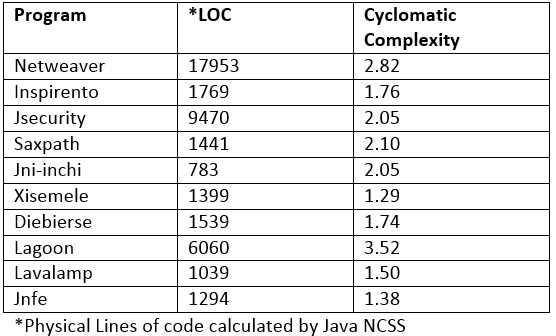
\includegraphics[width=\linewidth]{program_table}
\end{table}
%JACOB: Put in the text, not the table: "Physical lines of code calculated by JavaNCSS

\begin{figure}[!t]
\centering
  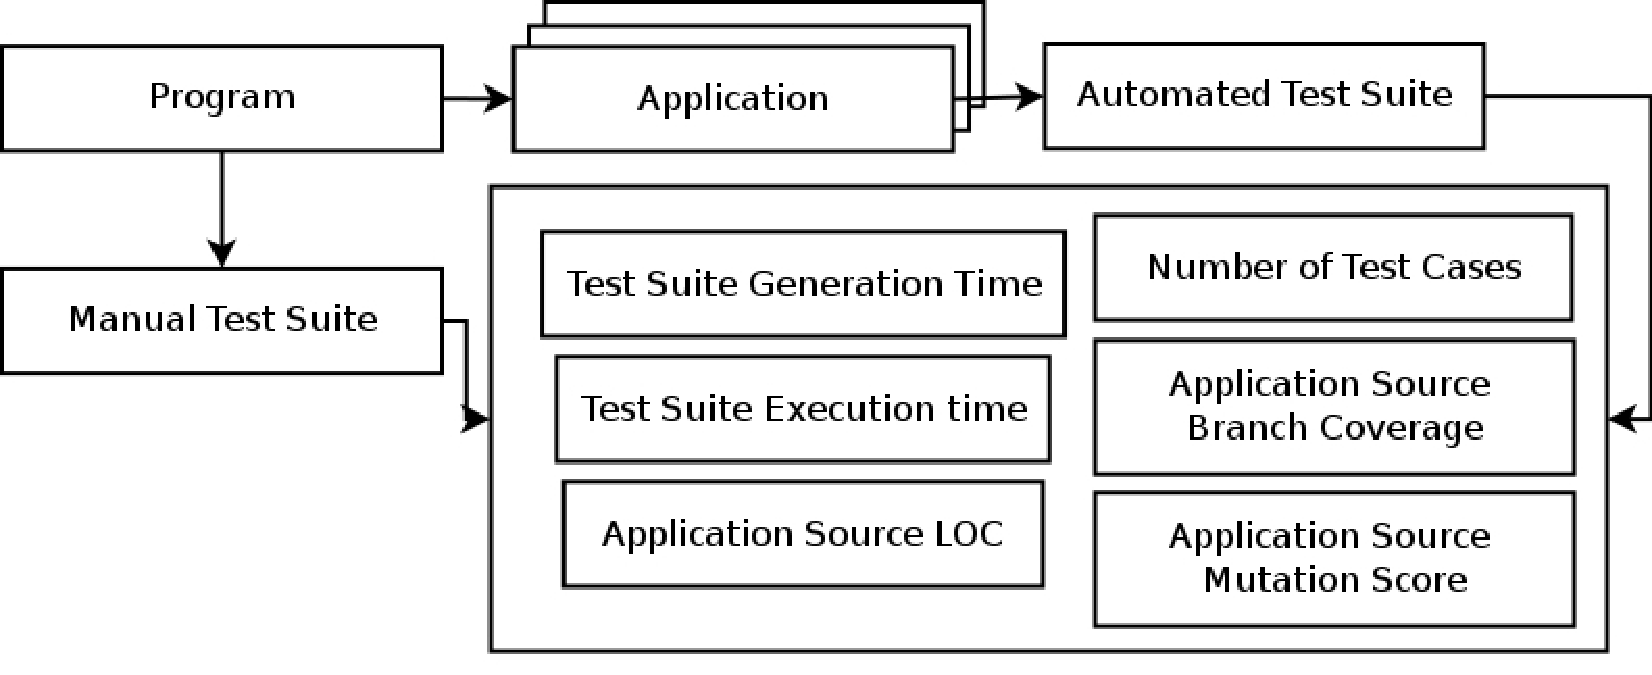
\includegraphics[width=\linewidth]{proccess_diagram}
    \caption{Test and Mutation Process}
  \label{fig:process_diagram}
\end{figure}


%----------------------------------------------------------------------------------------------------------------------------------------------------------------------------------------------------------------------------------
\subsection{Experiments and Results}
%----------------------------------------------------------------------------------------------------------------------------------------------------------------------------------------------------------------------------------

In our experiments, we first evaluated the time to create each test suite in comparison between Evosuite and CodePro. As shown in figure ~\ref{fig:Time}, CodePro generated test suites much more quickly than Evosuite did. Although Evosuite consistently takes longer to generate tests regardless of number lines of code and the complexity of the test suite. However, once we compare the complexity of the source code to the time to generate and the complexity of the test suites themselves, there is a clear trade off between time and complexity.

\begin{figure}[!t]
\centering
  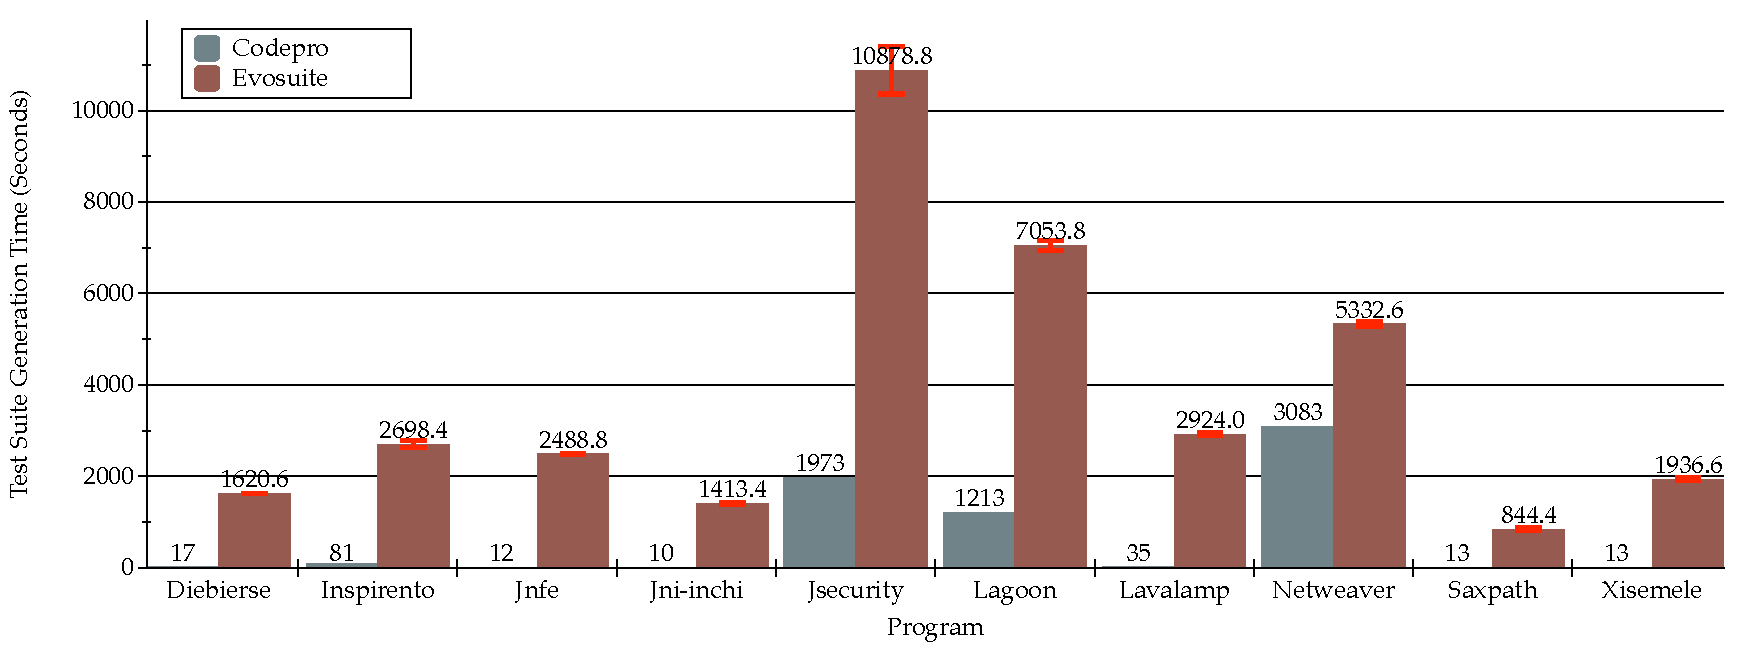
\includegraphics[width=\linewidth]{Time}
    \caption{Time to Generate Test Suite}
  \label{fig:Time}
\end{figure}

\begin{figure*}[!t]
\centering
  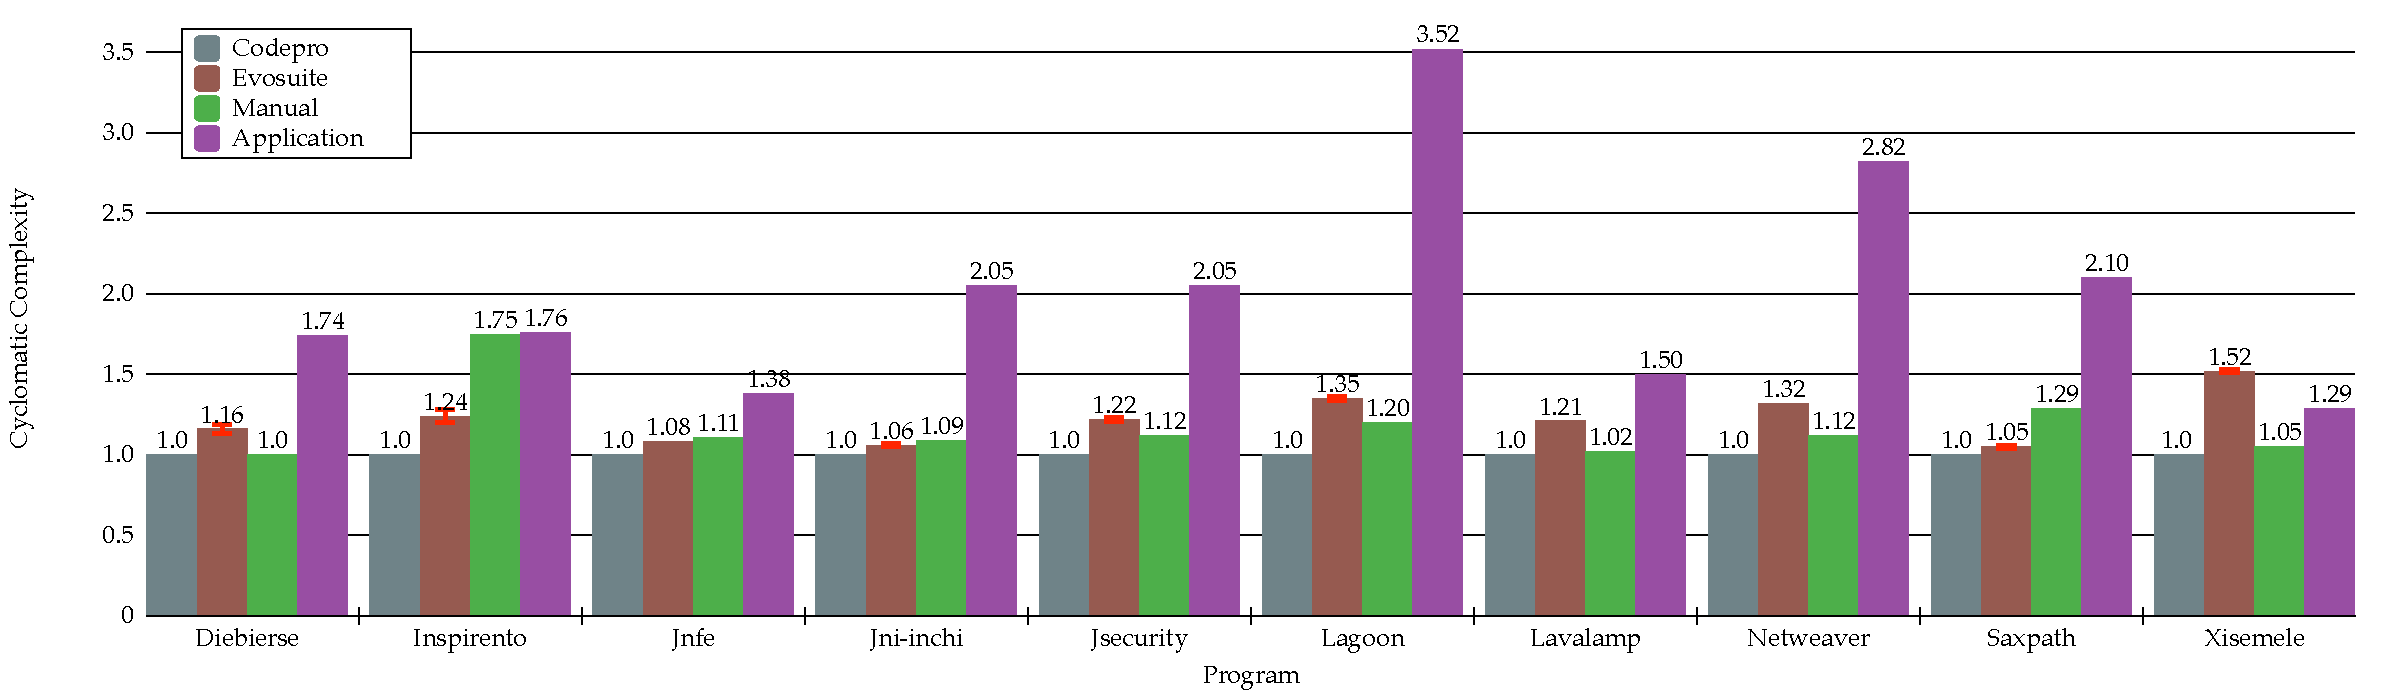
\includegraphics[width=\linewidth]{Complexity}
   \caption{Cyclomatic Complexity of Test Suites and Source Code}
  \label{fig:Complexity}
\end{figure*}

In figure~\ref{fig:Complexity}, we list the complexities of the source code of the program, and the generated test suites from manual, Evosuite, and Codepro. Note that more complex tests can be more difficult to maintain. The Evosuite test suites are generally more complex than the other two, whereas CodePro is consistently at a lower complexity level. Due to increased complexity of the test suites, it can take more time create and run them~\cite{alspaugh:2007}. As evidenced by figure~\ref{fig:Time_Complexity}, this indeed seems to be the case. In this data set, it would seem that the more complex the source code is, the more complex the tests are. Furthermore, the more complex the tests are, the longer the test generation takes to complete. This figure displays the complexity of the test suite versus the time it took to generate the test suite. 

\begin{figure*}[!t]
\centering
  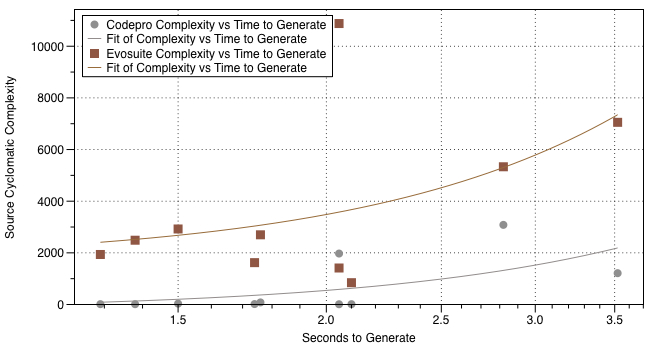
\includegraphics[width=\textwidth]{Time_Complexity}
    \caption{Time to Generate vs. Test Suite Cyclomatic Complexity}
  \label{fig:Time_Complexity}
\end{figure*}


CodePro maintains a low complexity level, but in doing so, this may lead to an inability to address complex code that requires deeper test cases. Although there is a performance boost in the speed to generate the test cases, one must also further examine the quality of the tests that are generated. Evosuite is more complex than the manually generated tests, which may mean that Evosuite cover deeper cases. If the depth of the tests are deeper in Evosuite, than one would expect the mutation scores to increase because the quality of tests would be higher. 

Using mutation scores as a measurement for quality of the tests, we then observe the overall mutation scores given to manual, Evosuite, and CodePro test suites in figure~\ref{fig:Mutation_Score}. Manual tests generate higher mutation scores in four of the programs, whereas Evosuite also receives higher mutations scores for half of the programs. CodePro receives the highest mutation score for one of the programs by a small margin, but for the rest of the test suites, the scores are the lowest by a large gap. Only in Diebierse did Evosuite vary greatly in the scores received. This indicates that although the average mutation score for Evosuite is within a more unpredictable range of results in one case, on average Evosuite can match the mutation score and quality of the manually written tests.

\begin{figure*}[!t]
\centering
  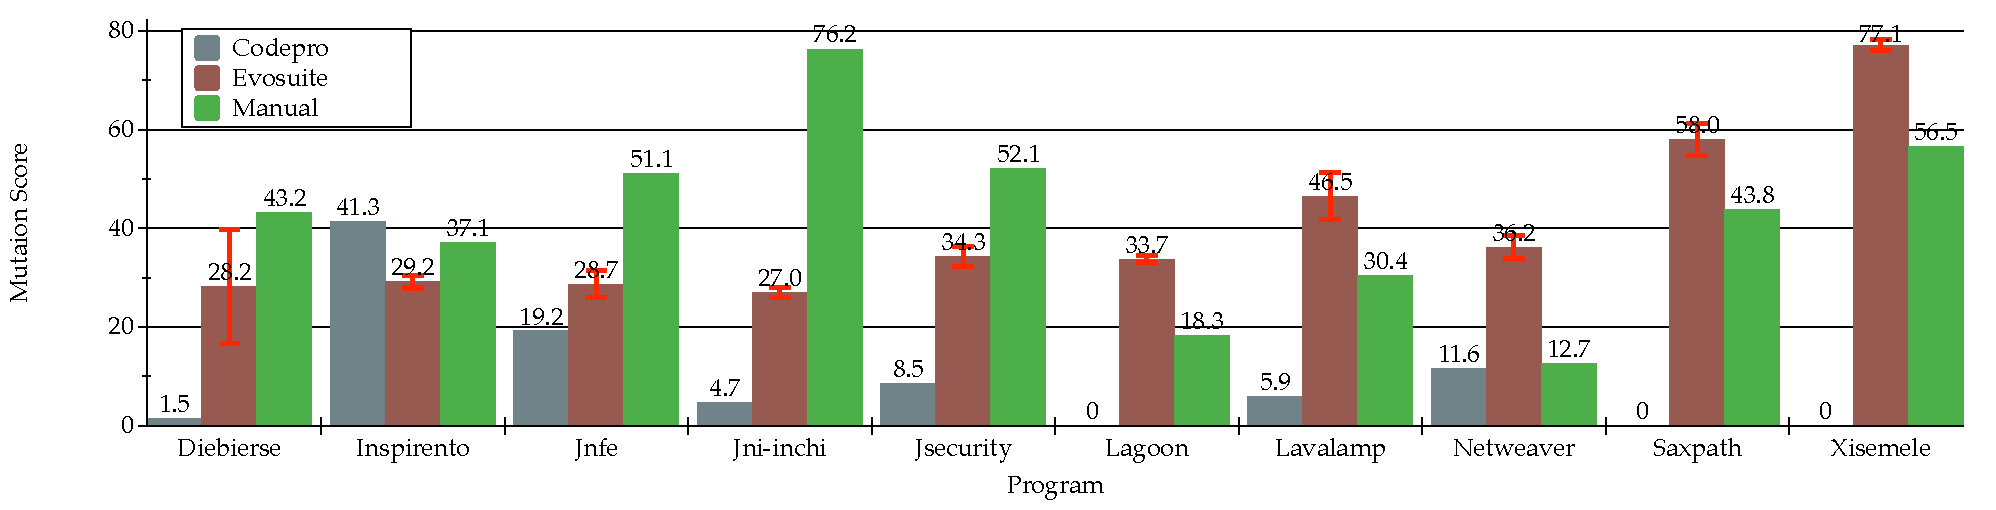
\includegraphics[width=\textwidth]{Mutation_Score}
    \caption{Mutation Score}
  \label{fig:Mutation_Score}
\end{figure*}

To further examine the cause of this, we look at figure~\ref{fig:Complexity_Mutation}, which describes the relationships between the mutation score of the test suites and the complexities of the source code. Notice that the manually written tests retain the highest mutation score overall at first. As the complexity of the program increases over time, the the mutation score begins to drop. Around a cyclomatic complexity of 2.3, we find that Evosuite's retains a higher mutation score than manually written tests. CodePro overall receives abysmal mutation scores, and as the cyclomatic complexity of the program increases, the mutation score drops to 0.

This graph is an eye opener to the reality of capturing deeper test cases. Up until a certain point human beings can write deeper test cases to more complex functions. Once the programs become complex, it may be too difficult for a person to cover complex parts of code that require deeper test cases. Evosuite may be at an advantage with its learning algorithm that modifies itself over time to improve the mutation score. With Evosuite seeming to edge out the other two methods in terms of depth, one must also examine the breadth each of the tools can cover as well.

\begin{figure*}[!t]
\centering
  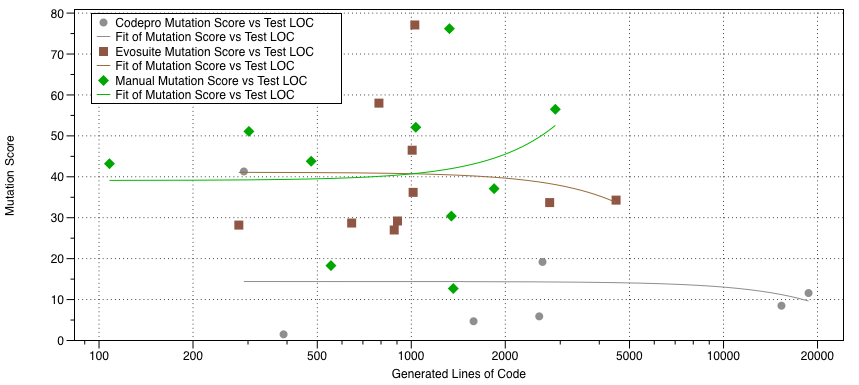
\includegraphics[width=\textwidth]{LOC_Mutation}
    \caption{LOC vs. Mutation Score}
  \label{fig:LOC_Mutation}
\end{figure*}


In figure~\ref{fig:LOC_Mutation} the relationship between lines of code of the test suite and and mutation score gives an initial impression that automated test suites lack the efficiency of a manually written test suite. CodePro not only results in the lowest mutation scores, but also creates the largest test suites. In our research, we found many of the test cases generated by CodePro were empty and contained comments for developers to put tests into templates. This reveals a different function that CodePro, unlike Evosuite, may be able to provide to developers. 

Although at first glance one may assume that CodePro lacks any usefulness because the quality of tests are low, one could also say that the templates provided by CodePro may give developers the flexibility of modifying and improving the test suite. Evosuite tests are much more complex, and could be conceivably difficult to maintain if the developers wished to evolve the test suite on their own. The trade off between automated and manually written tests could be an argument of modifiability in this case. Although Evosuite scores close to manually written tests when it comes to quality, how would one go about improving the test suites to meet that level depth that manual tests cover in larger programs? The tests would need to be modifiable from a human perspective, which in this case, could be an issue with tests suites like Evosuite.

\begin{figure*}[!t]
\centering
  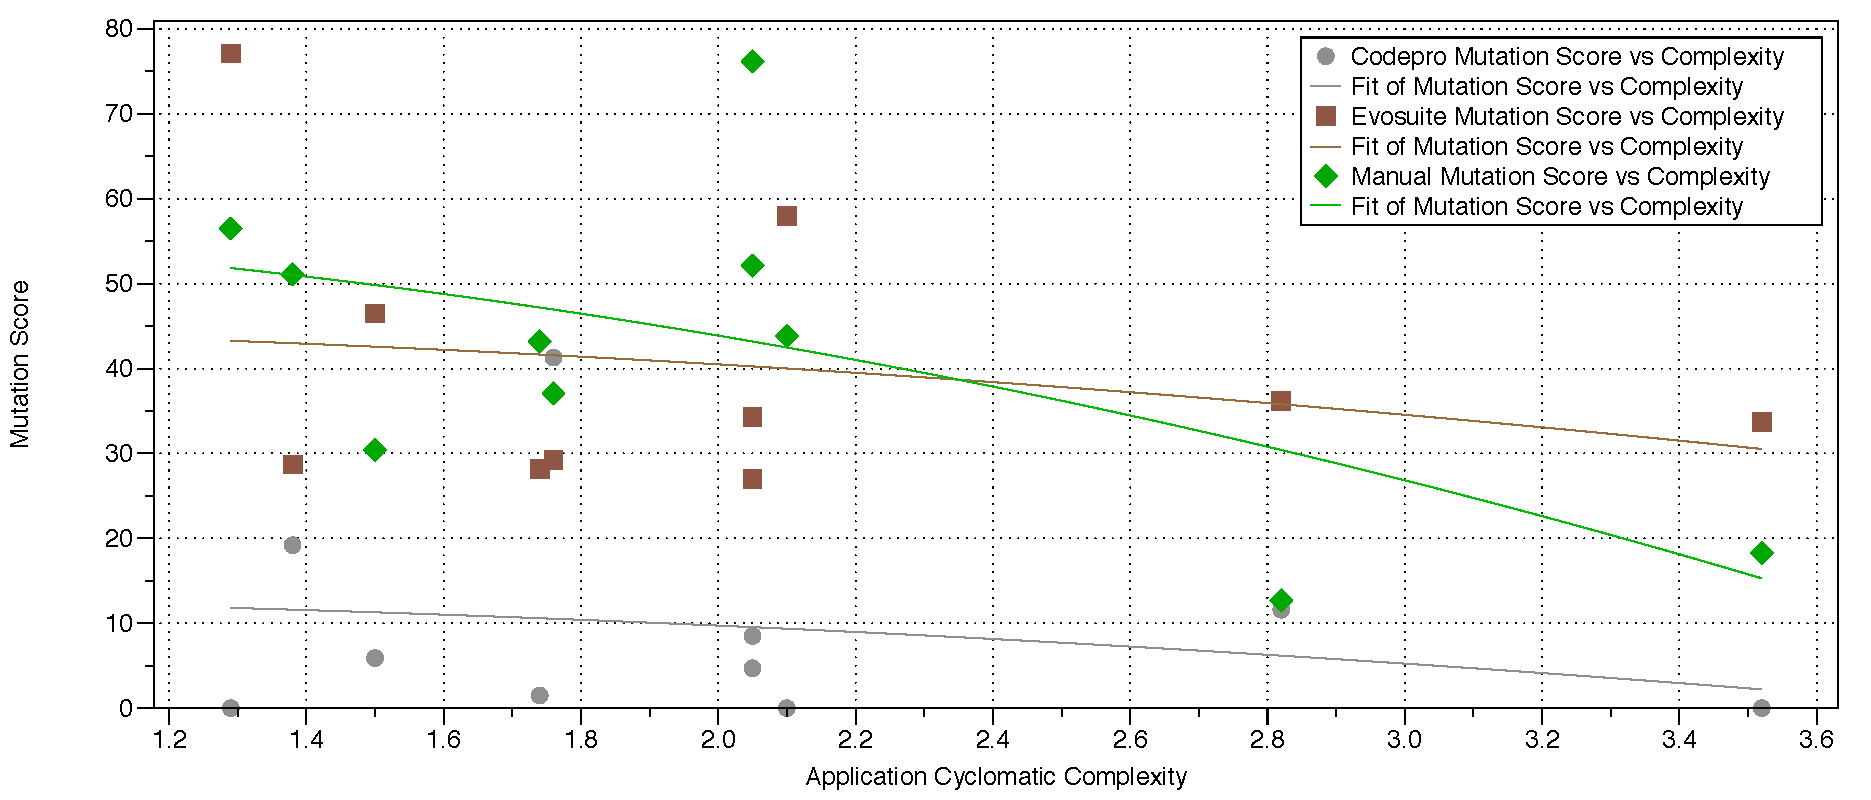
\includegraphics[width=\textwidth]{Complexity_Mutation}
    \caption{Mutation Score vs. Complexity}
  \label{fig:Complexity_Mutation}
\end{figure*}


Depth is important when evaluating the quality of tests, but breadth is an area one must consider when quantifying quality as well, as a test suite that deeply covers just one function will result in little breadth. In figure~\ref{fig:Coverage}, we find an extreme diversity of branch coverage amongst the three evaluated test suites. Overall, CodePro actually scores higher in branch coverage for four of the programs that were tested. Evosuite and the manually generated tests are tied for three programs in scoring the highest branch coverage. For the automated test generators, the branch coverages are closer on average, but manually written test suite scores seem to vary greatly. Again, this is probably due to the inconsistencies in different developers writing their test suites. For example, the developers on Lavalamp could have focused on a TDD philosophy in development, which would predictably yield higher test coverage. However, the developers for Netweaver may have only been concerned with testing one part of their code, and thus branch coverage remained low. In fact, unit tests for only complex parts of the code are common in development, and thus this chart alone only reveals the inconsistent nature of how developers write unit tests. One must look further at the mutation the branch coverage to reach a more definitive 

\begin{figure*}[!t]
\centering
  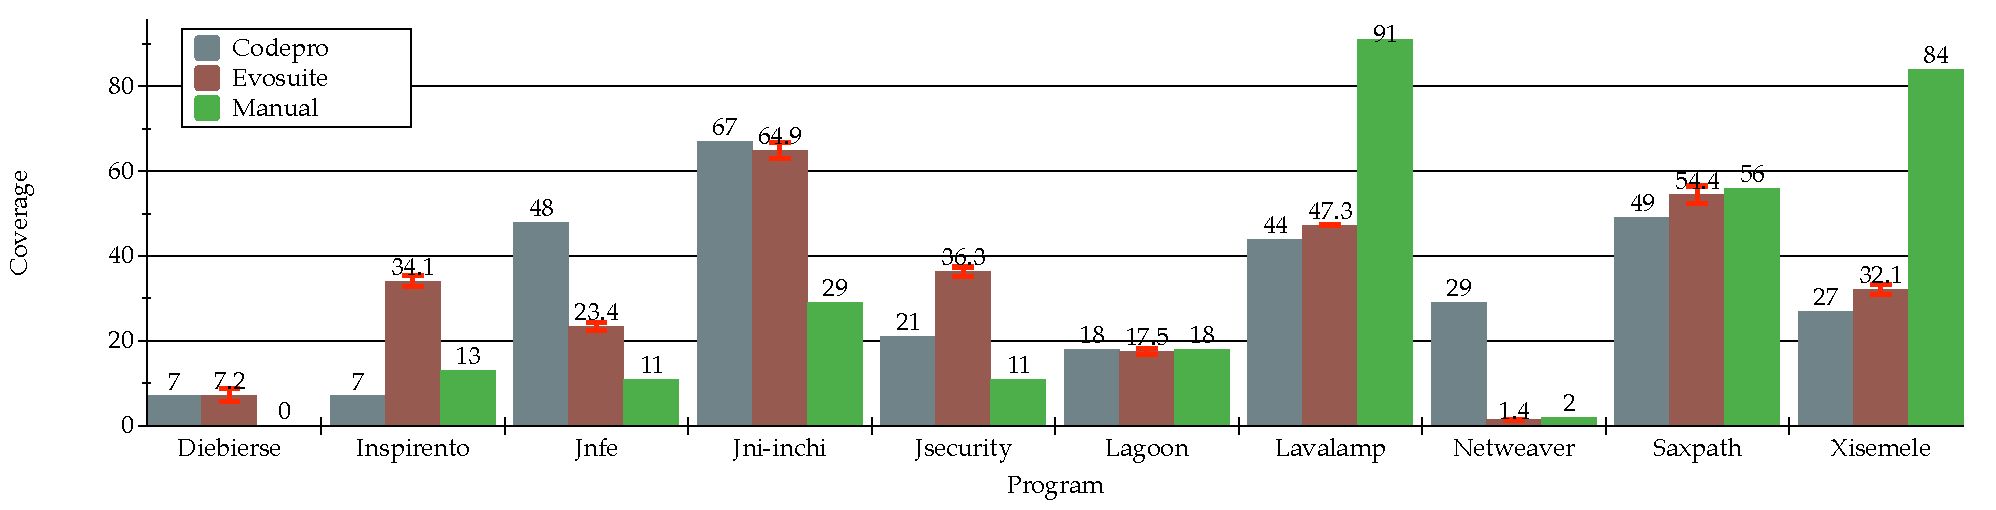
\includegraphics[width=\textwidth]{Coverage}
    \caption{Coverage}
  \label{fig:Coverage}
\end{figure*}

Finally we arrive at the center piece of the results, in comparing our evaluation of mutation scores and branch coverage. In figure~\ref{fig:Coverage_Mutation}, we compare the mutation score (depth) to the branch coverage (breadth) of the test suites. CodePro falls short in the mutation scores, but does have higher branch coverage coverage scores. As the branch coverage increases however, the mutation score in CodePro dips drastically. Understanding that the mutation score was never good to begin with in CodePro, this leads us back to the discussion in perhaps using CodePro as template tool rather than a upfront ready-to-go test suite. Although the mutation scores are low, the coverage is high, providing a large amount of tests for developers to look at and fill over time. 

More interesting are the similar trends between manual and Evosuite generated test suites. Initially Evosuite begins a bit lower in mutation score and branch coverage, but as the branch coverage increases, it would seem that Evosuite surpasses the Manual tests in quality. Overall, the quality of manual tests seems to rise above Evosuite ever so slightly. However, the trends seems to indicate that Evosuite will generate tests that will cover more code with better quality than manually written test suites, although both systems increase in quality as the test branch increases.



\begin{figure*}[!t]
\centering
  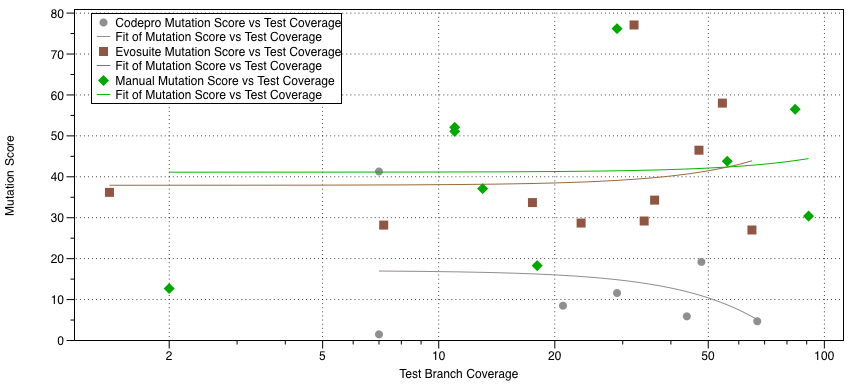
\includegraphics[width=\textwidth]{Coverage_Mutation}
    \caption{Coverage vs. Mutation}
  \label{fig:Coverage_Mutation}
\end{figure*}






\subsection{Threats to Validity}
Measurements in quality of software tests is a subjective measurement. Although mutation score is one way to measure the quality of a test suite, ignoring the human elements of tests are nigh impossible. Developers may need to view tests in order to diagnose faults in the code, and if a developer cannot understand the test they are reading, then the cost of time and effort could be increased on the human part.

The statistical analysis also may be a threat to validity, as the inconsistency in how both Evosuite and manually written tests are created. Also, CodePro generated some test suites with a mutation score of 0, which could mislead one to believing that CodePro has no use for creating quality tests. For this reason we remove these results to give a better impression of the trend CodePro test suites.

%----------------------------------------------------------------------------------------------------------------------------------------------------------------------------------------------------------------------------------
\section{Related Work}
%----------------------------------------------------------------------------------------------------------------------------------------------------------------------------------------------------------------------------------
There are few studies comparing the quality of manual and automated test suites. In one study researchers found that using automated test generation tools did not improve the ability to test the software ~\cite{Fraser:2013:AWT:2483760.2483774}. However, the study does not measure the quality of manual and automated generated test suites directly. Furthermore, only Evosuite is used to evaluate the mutations and generate the tests. Our research expands upon the question of the usefulness of automated generated test suites, and if certain systems in generating test suites work better than others.



%----------------------------------------------------------------------------------------------------------------------------------------------------------------------------------------------------------------------------------
\section{Conclusions and Future Work}
%----------------------------------------------------------------------------------------------------------------------------------------------------------------------------------------------------------------------------------


\bibliographystyle{abbrv}
\bibliography{sample}

%\balancecolumns 

\end{document}
